\documentclass[11pt]{report}

\usepackage{epsf,amsfonts}
\usepackage{graphicx}
\usepackage{mathtools}

\begin{document}

\title{MPAS-Mesh Specifications and Definitions}
\author{MPAS Development Team}

\maketitle
\tableofcontents

%-----------------------------------------------------------------------

\chapter{Summary}


This document will describe the required fields for a MPAS mesh. In addition, it
will define required orderings when creating an MPAS mesh. These together
should fully describe the MPAS mesh type and allow users to more easily
understand what makes an MPAS mesh.

%-----------------------------------------------------------------------

\chapter{General Mesh Requirements}

This chapter defines the general requirements for all MPAS meshes. Along with specific requirements for different element types (cell, edge, vertex). These include ordering specifications for one type of element relative to another.

\begin{itemize}
	\item MPAS meshes must be defined using a right handed coordinate system.
	\item Spherical grids must be centered at (0,0,0).
	\item Two arrays that are both relative to the element type must be ordered in the exact same way if possible.
	\item Input meshes are required to have a time dimension that is the unlimited (record) dimension.
\end{itemize}

When creating an MPAS mesh, it is recommended to ensure the correct ordering
relative to edges, then vertices, then cells. Ordering things in this way
simplifies the process.

\section{Requirements relative to edges}

At a given edge, two vectors $\vec{u}$ and $\vec{v}$ are defined as the normal and tangential vectors, respectively. These are defined as:
\begin{equation}
	\vec{u} = cellsOnEdge(2, iEdge) - cellsOnEdge(1, iEdge)
\end{equation}
\begin{equation}
	\vec{v} = verticesOnEdge(2, iEdge) - verticesOnEdge(1, iEdge)
\end{equation}

\begin{itemize}
	\item The surface normal vector must be defined as $\vec{u} \times \vec{v}$.
	\item Angle edge must be the angle in radians $\vec{u}$ makes with the local eastward direction.
	\item edgesOnEdge must run counter-clockwise, beginning with the edges that surround cellsOnEdge(1, iEdge) and ending with the edges that surround cellsOnEdge(2, iEdge). \\
		  The current edge must be omitted from the list of edgesOnEdge, but can be assumed to be both the starting and ending position when checking for counter-clockwise ordering.
	\item weightsOnEdge must be ordered in exactly the same order as edgesOnEdge. i.e. weightsOnEdge(1, iEdge) can be assumed to apply to edgesOnEdge(1, iEdge).
\end{itemize}

\begin{figure}
	\centering
	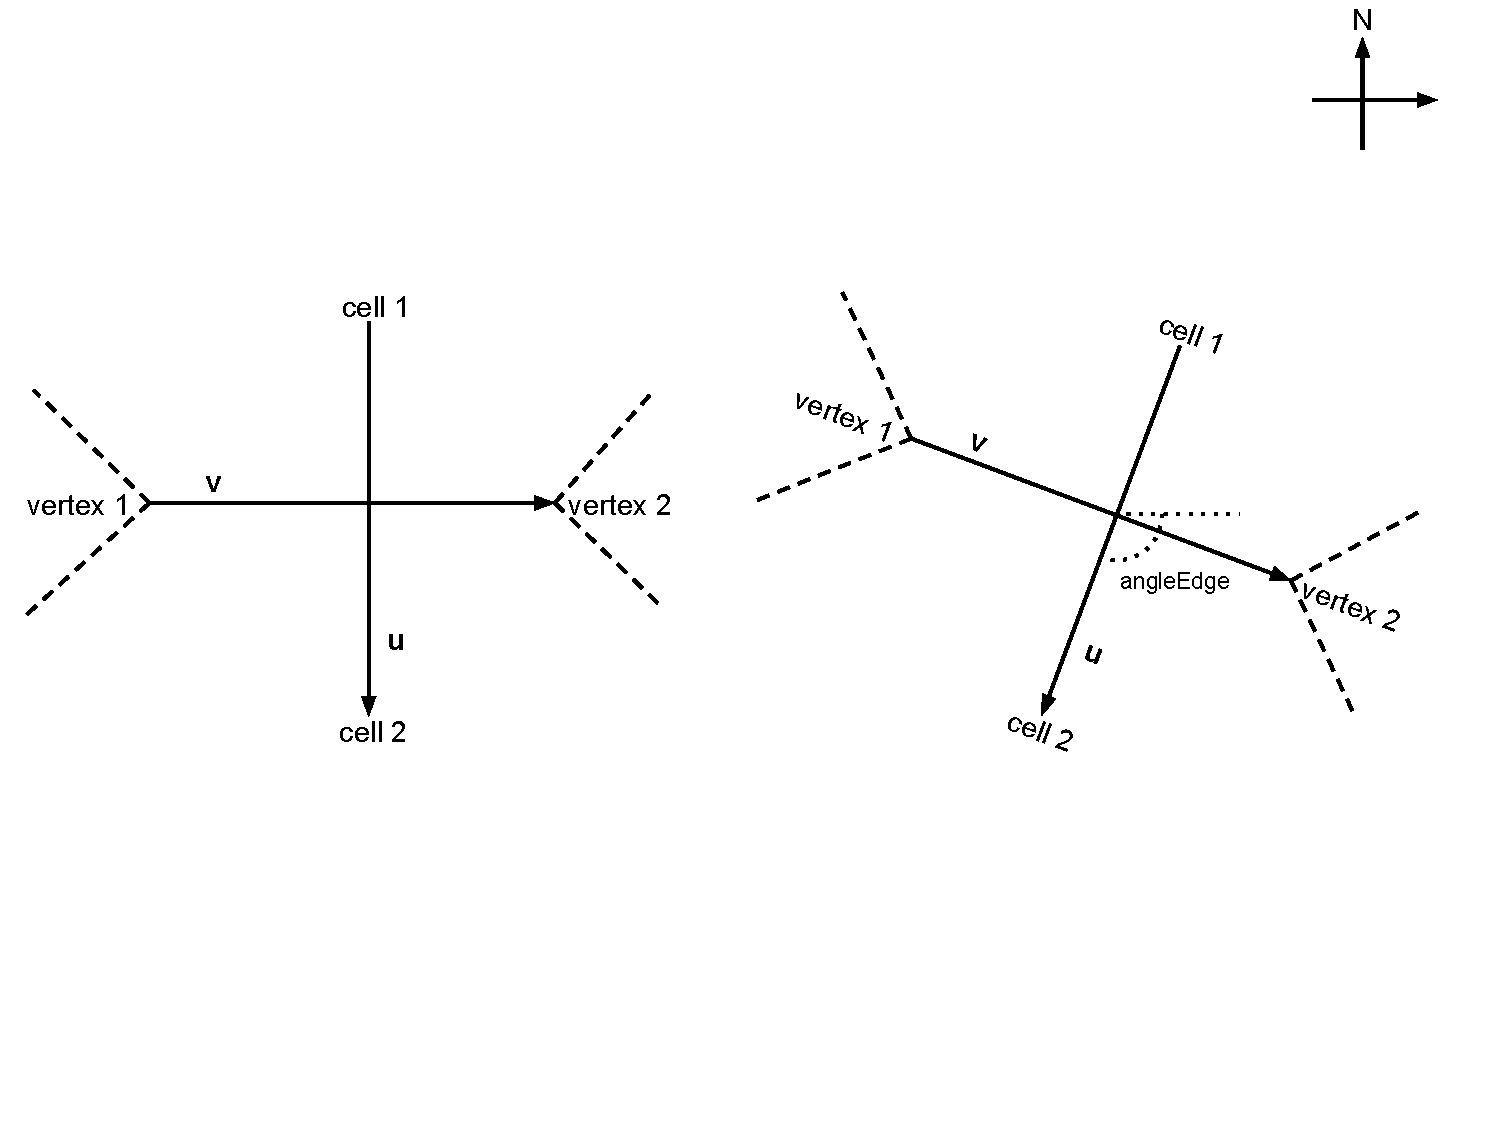
\includegraphics[scale=0.4]{figures/Edge Diagram.pdf}
	\caption{Ordering of elements relative to edges.}
\end{figure}

\begin{figure}
	\centering
	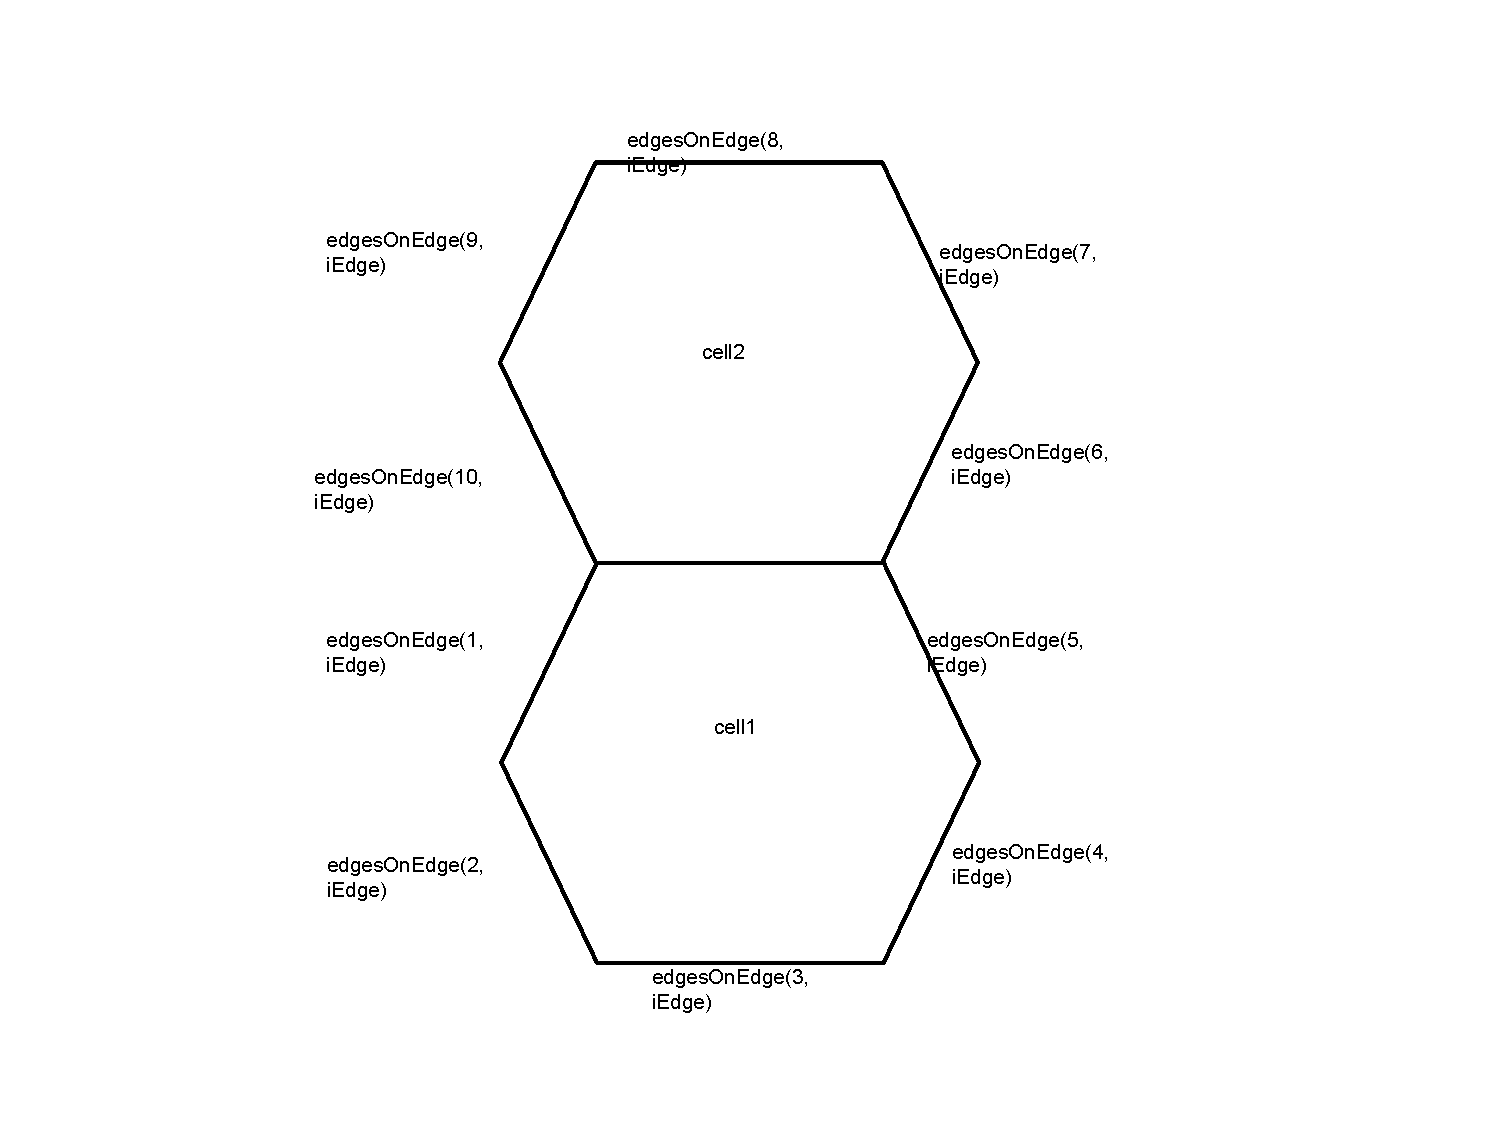
\includegraphics[scale=0.4]{figures/EdgeOnEdge Diagram.pdf}
	\caption{Ordering of edges relative to edges.}
\end{figure}

\section{Requirements relative to vertices}

\begin{itemize}
	\item Cells and Edges must run counter-clockwise around a given vertex.
	\item Edges must lead cells as they move around a vertex. \\
		  i.e. The vector defined by  \\
		  {\small $(cellsOnVertex(n, iVertex) - iVertex) \times (edgesOnVertex(n, iVertex) - iVertex)$} \\
		  must be surface normal, for all values of $n$.
	\item kiteAreasOnVertex(n, iVertex) is the intersection area of areaTriangle(iVertex) with areaCell(cellsOnVertex(n,iVertex)) for all values of $n$.
\end{itemize}

\begin{figure}
	\centering
	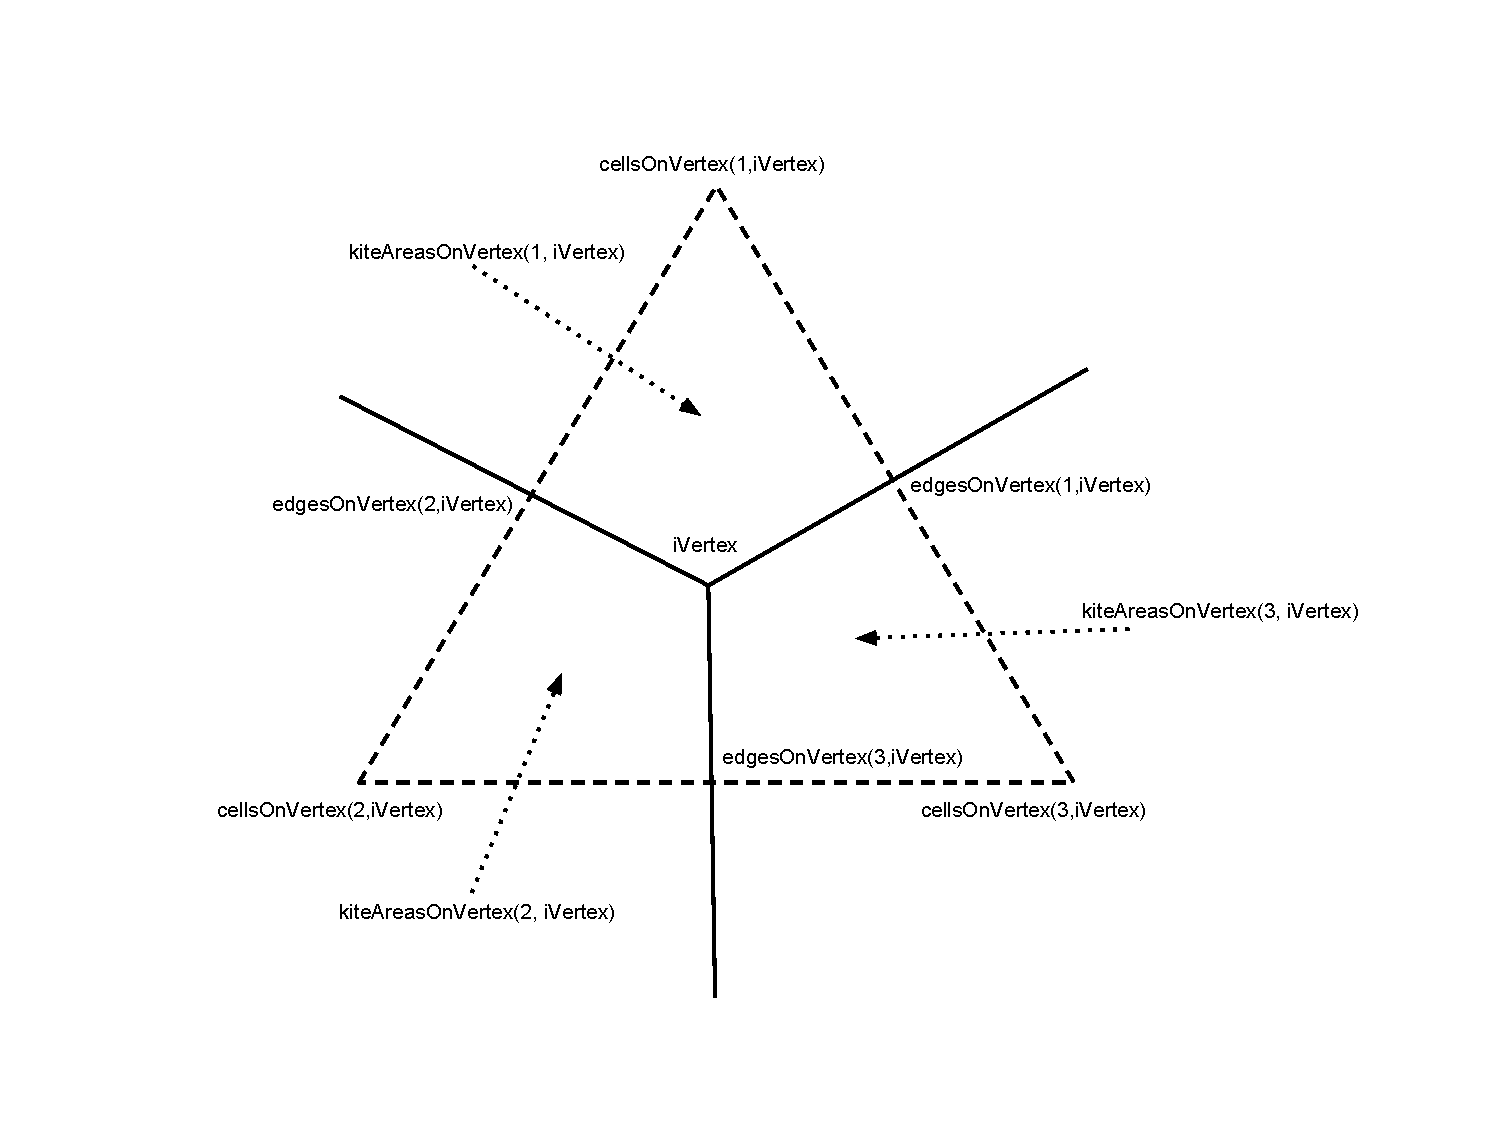
\includegraphics[scale=0.4]{figures/Vertex Diagram.pdf}
	\caption{Ordering of elements relative to vertices.}
\end{figure}

\section{Requirements relative to cells}

\begin{itemize}
	\item Cells, Edges, and Vertices all run counter-clockwise around a cell.
	\item The edge defined at edgesOnCell(n, iCell) must be on the edge between iCell and cellsOnCell(n, iCell) for all values of $n$.
	\item verticesOnCell(n, iCell) leads both edgesOnCell(n, iCell) and cellsOnCell(n, iCell) for all values of $n$. \\
		  i.e. The vector defined by \\
		  {\small $(edgesOnCell(n, iCell) - iCell) \times (verticesOnCell(n, iCell) - iCell)$} \\
		  must be surface normal for all values of $n$, or the substitution of cellsOnCell for edgesOnCell.
\end{itemize}

\begin{figure}
	\centering
	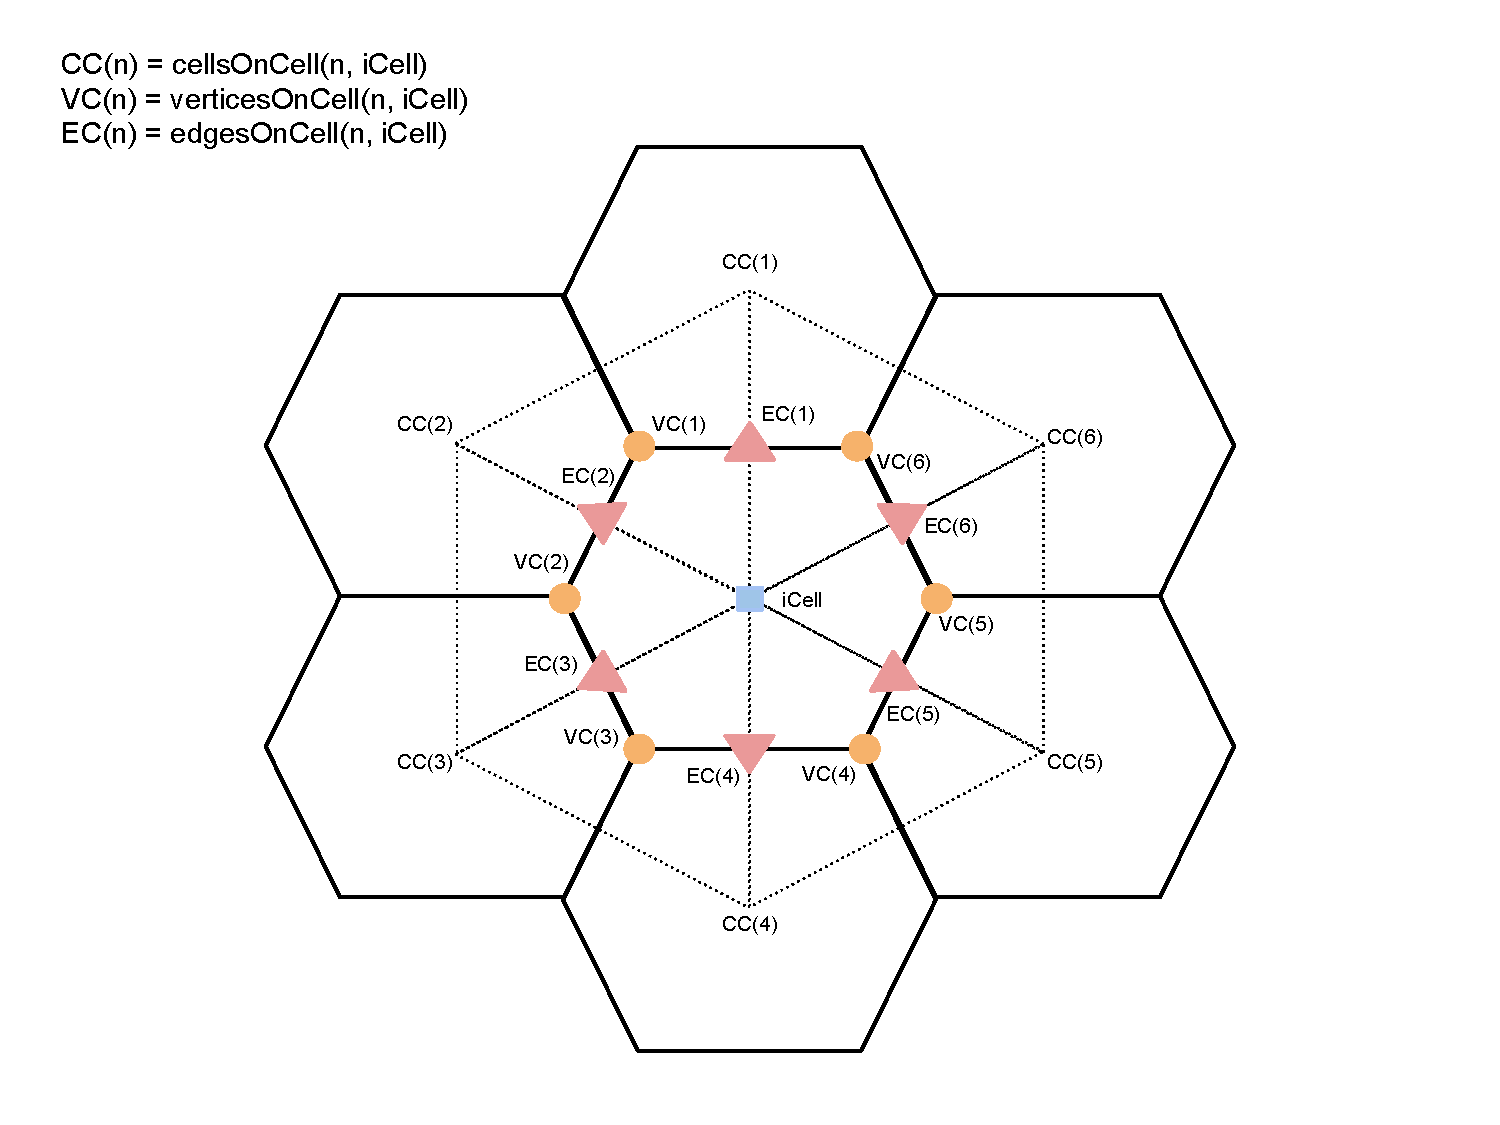
\includegraphics[scale=0.4]{figures/Cell Diagram.pdf}
	\caption{Ordering of elements relative to cells.}
\end{figure}

%-----------------------------------------------------------------------

\chapter{Requirements}

The following list of fields are required by all MPAS cores, and the MPAS framework assumes these fields exist.

\begin{itemize}
	\item latCell - Latitude in radians of all cell centers. Valid range of $-\frac{\pi}{2}$ to $\frac{\pi}{2}$.\\
		  Dimensions: nCells \\
		  Could be computed internally. 
	\item lonCell - Longitude in radians of all cell centers. Valid range of $0$ to $\pi$. \\
		  Dimensions: nCells \\
		  Could be computed internally. 
	\item xCell - x axis position of all cell centers. \\
		  Dimensions: nCells
	\item yCell - y axis position of all cell centers. \\
		  Dimensions: nCells
	\item zCell - z axis position of all cell centers. \\
		  Dimensions: nCells
	\item indexToCellID - Global cell ID for all cell centers. \\
		  Dimensions: nCells
	\item latEdge - Latitude in radians of all edge locations. Valid range of $-\frac{\pi}{2}$ to $\frac{\pi}{2}$. \\
		  Dimensions: nEdges
		  Could be computed internally. 
	\item lonEdge - Longitude in radians of all edge locations. Valid range of $0$ to $\pi$. \\
		  Dimensions: nEdges
		  Could be computed internally. 
	\item xEdge - x axis position of all edge locations. \\
		  Dimensions: nEdges
	\item yEdge - y axis position of all edge locations. \\
		  Dimensions: nEdges
	\item zEdge - z axis position of all edge locations. \\
		  Dimensions: nEdges
	\item indexToEdgeID - Global edge ID for all edge locations. \\
		  Dimensions: nEdges
	\item latVertex - Latitude in radians of all cell vertices. Valid range of $-\frac{\pi}{2}$ to $\frac{\pi}{2}$. \\
		  Dimensions: nVertices
		  Could be computed internally. 
	\item lonVertex - Longitude in radians of all cell vertices. Valid range of $0$ to $\pi$. \\
		  Dimensions: nVertices
		  Could be computed internally. 
	\item xVertex - x axis position of all cell vertices. \\
		  Dimensions: nVertices
	\item yVertex - y axis position of all cell vertices. \\
		  Dimensions: nVertices
	\item zVertex - z axis position of all cell vertices. \\
		  Dimensions: nVertices
	\item indexToVertexID - Global vertex ID for all cell vertices. \\
		  Dimensions: nVertices
	\item cellsOnEdge - Cell indices that saddle a given edge. \\
		  Dimensions: 2 * nEdges
	\item nEdgesOnCell - Number of edges on a given cell. \\
		  Dimensions: maxEdges * nCells
	\item nEdgesOnEdge - Number of edges on a given edge. Used to reconstruct tangential velocities. \\
		  Dimensions: maxEdges2 * nEdges
	\item edgesOnCell - Edge indices that surround a given cell. \\
		  Dimensions: maxEdges * nCells
	\item edgesOnEdge - Edge indices that are used to reconstruct tangential velocities. \\
		  Dimensions: maxEdges2 * nEdges
	\item weightsOnEdge - Weights used to reconstruct tangential velocities. \\
		  Dimensions: maxEdges2 * nEdges
		  Could be computed internally. 
	\item dvEdge - Distance in meters between the vertices that saddle a given edge. \\
		  Dimensions: nEdges
		  Could be computed internally. 
	\item dcEdge - Distance in meters between the cells that saddle a given edge. \\
		  Dimensions: nEdges
		  Could be computed internally. 
	\item angleEdge - Angle in radians an edge's normal vector makes with the local eastward direction. \\
		  Dimensions: nEdges
		  Could be computed internally. 
	\item areaCell - Area in square meters for a given cell of the primary mesh. \\
		  Dimensions: nCells
		  Could be computed internally. 
	\item areaTriangle - Area in square meters for a given triangle of the dual mesh. \\
		  Dimensions: nVertices
		  Could be computed internally. 
	\item edgeNormalVectors - Cartesian coordinates for the normal vector of a given edge. \\
		  Dimensions: 3 * nEdges
		  Could be computed internally. 
	\item edgeTangentVectors - Cartesian coordinates for the tangent vector of a given edge. \\
		  Dimensions: 3 * nEdges
		  Could be computed internally. 
	\item localVerticalUnitVectors - Unit surface normal vectors defined at a given cell. \\
		  Dimensions: 3 * nCells
		  Could be computed internally. 
	\item cellTangentPlane - The two vectors that define a tangent plane at a given cell. \\
		  Dimensions: 3 * 2 * nCells
		  Could be computed internally. 
	\item cellsOnCell - Cell indices that surround a given cell. \\
		  Dimensions: maxEdges * nCells
	\item verticesOnCell - Vertex indices that surround a given cell. \\
		  Dimensions: maxEdges * nCells
	\item verticesOnEdge - Vertex indices that saddle a given edge. \\
		  Dimensions: 2 * nEdges
	\item edgesOnVertex - Edge indices that radiate from a given vertex. \\
		  Dimensions: vertexDegree * nVertices
	\item cellsOnVertex - Cell indices that radiate from a given vertex. \\
		  Dimensions: vertexDegree * nVertices
	\item kiteAreasOnVertex - The intersection area of areaTriangle with each cell that radiates from a given vertex. \\
		  Dimensions: vertexDegree * nVertices
		  Could be computed internally. 
	\item coeffs\_reconstruct - Coefficients to reconstruct velocity vectors at cells centers. \\
		  Dimensions: 3 * maxEdges * nCells
		  Computed internally. 
\end{itemize}


\end{document}
